\documentclass[11pt,letterpaper]{article}

\usepackage[utf8]{inputenc}
\usepackage[T1]{fontenc}
\usepackage[spanish,es-nodecimaldot]{babel}
\usepackage[letterpaper,margin=2.2cm,headheight=15pt]{geometry}
\usepackage[protrusion=true,expansion=false]{microtype}
\usepackage{xcolor}
\usepackage{graphicx}
\usepackage{booktabs}
\usepackage{tabularx}
\usepackage{longtable}
\usepackage{array}
\usepackage{enumitem}
\usepackage{fancyhdr}
\usepackage{hyperref}
\usepackage{xurl}
\usepackage{listings}
\usepackage{float}

\ifdefined\pdfinfoomitdate\pdfinfoomitdate=1\fi
\ifdefined\pdftrailerid\pdftrailerid{}\fi
\ifdefined\pdfsuppressptexinfo\pdfsuppressptexinfo=15\fi

\definecolor{ugblue}{HTML}{006A8D}
\definecolor{deepgreen}{HTML}{123D3A}
\definecolor{softgray}{HTML}{F1F5F4}
\definecolor{midgray}{HTML}{5D6B6B}
\definecolor{warning}{HTML}{A45A00}
\definecolor{danger}{HTML}{8A1C1C}

\hypersetup{
  colorlinks=true,
  linkcolor=ugblue,
  urlcolor=ugblue,
  hypertexnames=false,
  pdftitle={Manual tecnico - Prototipo BI asistido por IA},
  pdfauthor={Emily Dayan Robles Alvarado y Lesly Samay Velasquez Anchundia}
}

\pagestyle{fancy}
\fancyhf{}
\lhead{Manual técnico}
\rhead{Prototipo BI asistido por IA}
\cfoot{\thepage}

\setlength{\parindent}{0pt}
\setlength{\parskip}{0.52em}
\setlist[itemize]{leftmargin=1.5em,itemsep=0.22em,topsep=0.3em}
\setlist[enumerate]{leftmargin=1.7em,itemsep=0.32em,topsep=0.35em}
\renewcommand{\arraystretch}{1.2}
\newcommand{\file}[1]{\texttt{#1}}
\newcommand{\warningbox}[1]{\begin{center}\fcolorbox{danger}{softgray}{\begin{minipage}{0.90\textwidth}\textcolor{danger}{\textbf{Precaución.}} #1\end{minipage}}\end{center}}
\newcommand{\notebox}[1]{\begin{center}\fcolorbox{ugblue}{softgray}{\begin{minipage}{0.90\textwidth}\textcolor{ugblue}{\textbf{Nota.}} #1\end{minipage}}\end{center}}

\lstdefinestyle{terminal}{
  basicstyle=\ttfamily\small,
  backgroundcolor=\color{softgray},
  frame=single,
  rulecolor=\color{midgray},
  breaklines=true,
  columns=fullflexible,
  keepspaces=true,
  showstringspaces=false,
  xleftmargin=0.4em,
  xrightmargin=0.4em,
  aboveskip=0.6em,
  belowskip=0.6em
}

\begin{document}
\hypersetup{pageanchor=false}

\begin{titlepage}
  \thispagestyle{empty}
  \vspace*{0.8cm}
  {\color{ugblue}\rule{\textwidth}{2.8pt}}
  \vspace{1.2cm}

  {\Large Universidad de Guayaquil\\[0.25em]
  Facultad de Ciencias Matemáticas y Físicas\\
  Carrera de Software}

  \vfill

  {\color{deepgreen}\fontsize{30}{35}\selectfont\textbf{Manual técnico}}\\[0.7em]
  {\LARGE Instalación, operación y réplica del entorno}\\[0.6em]
  {\large Prototipo web de inteligencia de negocios asistido por IA}

  \vspace{1.5cm}

  \begin{tabularx}{\textwidth}{@{}>{\bfseries}l X@{}}
    Autoras & Emily Dayan Robles Alvarado y Lesly Samay Velásquez Anchundia \\
    Versión del manual & 1.8.0 \\
    Línea base & Ramas \file{develop} y \file{main} \\
    Repositorio & \href{https://github.com/LFXAS/prototipo-bi-ia}{LFXAS/prototipo-bi-ia} \\
    Clasificación & Uso académico y técnico - repositorio público \\
    Fecha & 10 de septiembre de 2026 \\
  \end{tabularx}

  \vfill
  {\color{ugblue}\rule{\textwidth}{2.8pt}}
\end{titlepage}

\hypersetup{pageanchor=true}
\pagenumbering{roman}
\tableofcontents
\newpage
\pagenumbering{arabic}

\section{Propósito y audiencia}

Este manual permite instalar, levantar, comprobar, mantener y replicar el ambiente técnico del prototipo. Está dirigido a las autoras, docentes revisores, colaboradores autorizados y personal técnico que necesite reproducir la demostración.

El documento cubre tres modalidades:

\begin{enumerate}
  \item \textbf{Desarrollo desde el código}: clona el repositorio y construye las imágenes localmente.
  \item \textbf{Vista local de entrega}: añade Nginx en el puerto 8080 y reutiliza la API y las bases de desarrollo.
  \item \textbf{Ejecución de una entrega completa}: descarga imágenes de GitHub Container Registry (GHCR) en un proyecto Compose aislado.
\end{enumerate}

La versión actual conserva la infraestructura del Sprint 1 y el núcleo administrativo del Sprint 2: autenticación JWT, RBAC, auditoría y configuración LLM. El primer incremento del Sprint 3 añade parámetros tipados y la administración web de una fuente SQL Server con secreto cifrado, prueba de sólo lectura y activación única. Metadatos, ETL, datamart, dashboard, reportería y Copiloto BI continúan fuera de este incremento.

\section{Arquitectura operativa}

\begin{center}
\fcolorbox{ugblue}{softgray}{%
  \begin{minipage}{0.91\textwidth}
    \centering
    \textbf{Usuario} $\rightarrow$ \textbf{Frontend React/Vite o Nginx}\\[0.35em]
    $\downarrow$ peticiones \file{/api/}\\[0.35em]
    \textbf{Backend FastAPI}\\[0.35em]
    \begin{tabular}{c@{\hspace{1.6cm}}c}
      $\swarrow$ & $\searrow$ \\
      \textbf{PostgreSQL} & \textbf{SQL Server} \\
      \file{app} + \file{mart} & AdventureWorks 2022 \\
      lectura/escritura interna & usuario externo de sólo lectura
    \end{tabular}
  \end{minipage}}
\end{center}

\subsection{Servicios}

\begin{tabularx}{\textwidth}{@{}l X l l@{}}
  \toprule
  Servicio & Responsabilidad & Puerto desarrollo & Persistencia \\
  \midrule
  frontend & Interfaz React y proxy a la API & 5173 & Código y dependencias \\
  frontend-delivery & Frontend compilado servido por Nginx & 8080 & Sin volumen \\
  backend & API FastAPI, configuración y salud & 8000 & Código montado \\
  postgres & Configuración interna y futuro datamart & 55432 & Volumen \file{postgres\_data} \\
  sqlserver & Fuente AdventureWorks externa & 51433 & Volumen \file{sqlserver\_data} \\
  ollama & LLM local opcional, sólo red interna & No publicado & Volumen \file{ollama\_models} \\
  raíz criptográfica & Clave local para cifrar secretos autorizados & No aplica & Volumen \file{secret\_key\_data} \\
  \bottomrule
\end{tabularx}

Compose crea la red y los volúmenes de desarrollo bajo el nombre lógico \file{bi-ia-prototype}. El perfil \file{delivery} sólo añade Nginx a esa red; el perfil opcional \file{local-llm} añade Ollama sin publicar el puerto 11434 en el host. El volumen \file{secret\_key\_data} se monta exclusivamente en FastAPI. El Compose completo de entrega usa \file{bi-ia-prototype-release}, otra red, otros puertos y otros volúmenes. Ninguno usa contenedores PostgreSQL o SQL Server ajenos al proyecto.

\subsection{Estructura del repositorio}

\begin{lstlisting}[style=terminal]
backend/                  FastAPI, pruebas y migraciones
frontend/                 React, Vite, pruebas y Nginx
infra/postgres/           imagen e inicializacion PostgreSQL
infra/sqlserver/          imagen y restauracion AdventureWorks
infra/docs/               imagen reproducible de LaTeX
scripts/                  arranque, espera y verificacion
docs/                     arquitectura, guias y evidencias
.github/workflows/        integracion y entrega continuas
compose.yaml              entorno de desarrollo autocontenido
compose.release.yaml      entorno con imagenes de GHCR
Makefile                  comandos operativos abreviados
\end{lstlisting}

\section{Requisitos previos}

\subsection{Hardware recomendado}

\begin{itemize}
  \item Procesador de 64 bits con virtualización habilitada.
  \item 8 GB de memoria disponibles para Docker; 6 GB es el mínimo práctico.
  \item 15 GB libres para imágenes, capas, respaldo y volúmenes; reservar al menos 8 GB adicionales si se descargará el modelo local de Ollama.
  \item Conexión a Internet durante la primera construcción y restauración.
\end{itemize}

\subsection{Software requerido}

\begin{itemize}
  \item Docker Engine 24 o superior y Docker Compose v2; Docker Desktop es válido.
  \item Git para clonar y actualizar el repositorio.
  \item Acceso al repositorio público; permiso de escritura sólo para colaboradores autorizados.
  \item Para consumir imágenes públicas no se necesita iniciar sesión; si un paquete GHCR conserva visibilidad privada, se requieren credenciales con \file{read:packages}.
\end{itemize}

No se requiere instalar Python, Node.js, PostgreSQL, SQL Server, controladores ODBC ni LaTeX en el host.

En equipos ARM, incluido Apple Silicon, SQL Server usa \file{linux/amd64} mediante emulación. El primer arranque puede ser más lento.

\section{Configuración segura}

\subsection{Archivo de entorno}

El archivo \file{.env} contiene la configuración local y nunca debe enviarse a Git. Se crea desde el ejemplo:

\begin{lstlisting}[style=terminal,language=bash]
cp .env.example .env
\end{lstlisting}

Se deben reemplazar todos los valores que empiecen con \file{ChangeMe\_*}. Las claves deben cumplir la política de SQL Server: longitud suficiente y combinación de mayúsculas, minúsculas, números y símbolos.

\begin{longtable}{@{}p{0.31\textwidth}p{0.23\textwidth}p{0.38\textwidth}@{}}
  \toprule
  \textbf{Variable} & \textbf{Valor inicial} & \textbf{Uso} \\
  \midrule
  \endfirsthead
  \toprule
  \textbf{Variable} & \textbf{Valor inicial} & \textbf{Uso} \\
  \midrule
  \endhead
  \file{COMPOSE\_PROJECT\_NAME} & \file{bi-ia-prototype} & Prefijo aislado de red, contenedores y volúmenes. \\
  \file{FRONTEND\_PORT} & 5173 & Puerto web de desarrollo; 8080 en la entrega completa. \\
  \file{DELIVERY\_FRONTEND\_PORT} & 8080 & Vista Nginx que convive con Vite. \\
  \file{BACKEND\_PORT} & 8000 & Puerto de FastAPI y OpenAPI. \\
  \file{LOCAL\_POSTGRES\_PORT} & 55432 & Publicación local de PostgreSQL. \\
  \file{LOCAL\_SQLSERVER\_PORT} & 51433 & Publicación local de SQL Server. \\
  \file{POSTGRES\_DB} & \file{bi\_prototype} & Base interna y futuro datamart. \\
  \file{POSTGRES\_USER} & \file{bi\_app} & Cuenta de la aplicación interna. \\
  \file{POSTGRES\_PASSWORD} & secreto local & Clave de PostgreSQL. \\
  \file{SQLSERVER\_DATABASE} & \file{AdventureWorks2022} & Base externa restaurada. \\
  \file{SQLSERVER\_USER} & \file{bi\_reader} & Cuenta exclusiva de lectura. \\
  \file{SQLSERVER\_PASSWORD} & secreto local & Clave del lector. \\
  \file{SQLSERVER\_SA\_PASSWORD} & secreto local & Clave administrativa usada sólo durante inicialización. \\
  \file{IMAGE\_PREFIX} & ruta GHCR & Prefijo de las imágenes publicadas. \\
  \file{IMAGE\_TAG} & \file{main} & Entrega a ejecutar; se recomienda una etiqueta versionada. \\
  Credencial Gemini/Qwen & interfaz web & Se registra o reemplaza desde Configuración LLM; no pertenece a \file{.env}. \\
  \file{OLLAMA\_MODEL} & \file{qwen2.5:3b} & Modelo local ágil que se descarga explícitamente por equipo. \\
  \file{OLLAMA\_CONTEXT\_LENGTH} & 2048 & Límite local de contexto para controlar consumo de memoria y priorizar agilidad. \\
  \bottomrule
\end{longtable}

\warningbox{No copiar contraseñas, tokens, archivos \file{.env}, respaldos \file{.bak} ni volúmenes al repositorio. Ante una exposición, rotar inmediatamente la credencial y revisar el historial.}

\section{Instalación de desarrollo en este computador}

El proyecto se encuentra en \file{/home/ceo/Proyectos/BI}. Para una primera ejecución:

\begin{lstlisting}[style=terminal,language=bash]
cd "/home/ceo/Proyectos/BI"
cp .env.example .env
# Editar .env y cambiar todos los secretos ChangeMe_*
make bootstrap
\end{lstlisting}

\file{make bootstrap} realiza las siguientes acciones:

\begin{enumerate}
  \item valida o crea el archivo de configuración local;
  \item construye las imágenes propias;
  \item crea una red y tres volúmenes exclusivos;
  \item inicia PostgreSQL y espera su estado saludable;
  \item inicia SQL Server, descarga y restaura AdventureWorks si el volumen está vacío;
  \item crea y prueba el usuario \file{bi\_reader};
  \item aplica las migraciones Alembic pendientes;
  \item ejecuta el servicio \file{seed}, que incorpora sin duplicar el catálogo protegido aprobado;
  \item inicia FastAPI y después React;
  \item espera hasta que los cuatro servicios respondan correctamente.
\end{enumerate}

El primer arranque puede tardar varios minutos. Para observar la restauración:

\begin{lstlisting}[style=terminal,language=bash]
docker compose logs -f sqlserver
\end{lstlisting}

\section{Instalación en otro computador desde el código}

\subsection{Obtener el repositorio}

El código puede clonarse sin invitación porque el repositorio es público. Para crear ramas en el repositorio central, revisar o fusionar cambios se requiere ser colaborador autorizado.

\begin{lstlisting}[style=terminal,language=bash]
git clone https://github.com/LFXAS/prototipo-bi-ia.git
cd prototipo-bi-ia
\end{lstlisting}

La carpeta puede ubicarse en cualquier ruta; Compose utiliza rutas relativas.

\subsection{Preparar secretos}

\begin{lstlisting}[style=terminal,language=bash]
cp .env.example .env
# Abrir .env y reemplazar todos los valores ChangeMe_*
\end{lstlisting}

Si alguno de los puertos está ocupado, cambiarlo en \file{.env} antes del arranque.

\subsection{Construir y levantar}

\begin{lstlisting}[style=terminal,language=bash]
make bootstrap
\end{lstlisting}

\subsection{Confirmar el estado}

\begin{lstlisting}[style=terminal,language=bash]
docker compose ps
curl http://localhost:8000/api/v1/health/live
curl http://localhost:8000/api/v1/health/ready
\end{lstlisting}

Las dos respuestas deben indicar \file{"status":"ok"}; la segunda también debe indicar \file{"postgres":"ok"}.

\subsection{Abrir la aplicación}

\begin{itemize}
  \item Frontend: \url{http://localhost:5173}
  \item API: \url{http://localhost:8000}
  \item OpenAPI: \url{http://localhost:8000/docs}
\end{itemize}

\begin{figure}[H]
  \centering
  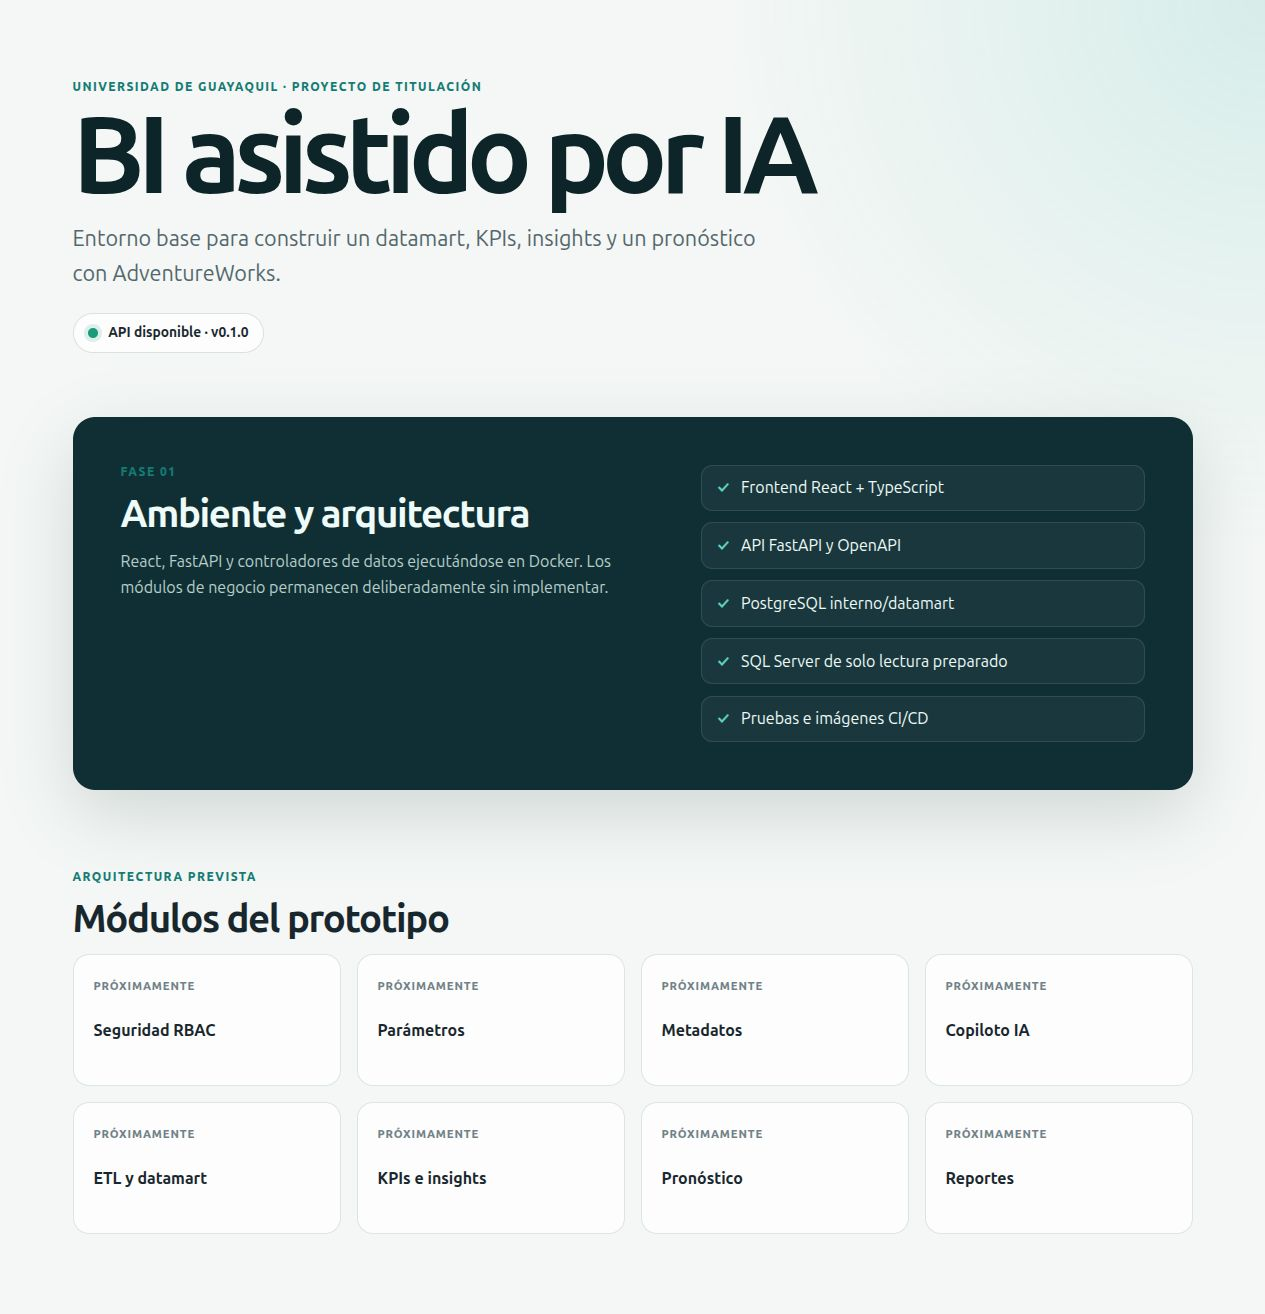
\includegraphics[width=0.88\textwidth]{../assets/sprint-01/frontend.jpg}
  \caption{Resultado esperado después de levantar el entorno de desarrollo.}
\end{figure}

\section{Vista local de entrega sin reemplazar desarrollo}

Con los servicios de desarrollo activos, ejecutar:

\begin{lstlisting}[style=terminal,language=bash]
make delivery-preview-up
\end{lstlisting}

El comando construye la etapa \file{production} del frontend y añade \file{frontend-delivery} mediante el perfil Compose \file{delivery}. No detiene Vite, no recrea el backend y no duplica PostgreSQL ni SQL Server.

\begin{itemize}
  \item Vite y recarga automática: \url{http://localhost:5173}
  \item Frontend compilado con Nginx: \url{http://localhost:8080}
  \item API compartida: \url{http://localhost:8000}
\end{itemize}

Esta modalidad valida el frontend que se empaquetará, pero no representa un ambiente productivo totalmente independiente porque comparte el backend de desarrollo.

\section{Operación funcional del Sprint 2}

El Sprint 2 se opera sobre el mismo ambiente levantado con \file{make bootstrap} o \file{make up}. No se crea una instalación ni un conjunto de contenedores adicional para seguridad: React, FastAPI y PostgreSQL ya contienen el incremento. La migración se aplica mediante el servicio \file{migrate}; después, el servicio \file{seed} carga de forma idempotente el catálogo protegido antes de iniciar FastAPI.

\subsection{Migraciones y datos semilla por equipo}

Cada volumen PostgreSQL pertenece exclusivamente al equipo que lo creó y nunca se transmite por GitHub. Cuando una programadora actualiza \file{develop} y levanta Compose, Alembic aplica el cambio de estructura y \file{seed} incorpora o actualiza los permisos, menús, rol administrador y cuenta inicial aprobados. Este orden permite que una base vacía quede operativa y que una base ya existente conserve sus datos locales no protegidos.

Para repetir sólo el catálogo base, sin borrar ni exportar PostgreSQL, se ejecuta desde la raíz del repositorio:

\begin{lstlisting}[style=terminal,language=bash]
make seed
\end{lstlisting}

La operación no duplica registros. No distribuye cuentas temporales, auditoría, contraseñas, tokens, configuraciones LLM ni datos de negocio. Una semilla demostrativa futura deberá ser sintética, opcional y aprobada con la especificación del módulo que la consuma.

\subsection{Acceso inicial y sesión}

El primer arranque crea la cuenta administradora inicial desde las variables de administración definidas en \file{.env}. Estos valores son secretos locales: se cambian antes de una demostración compartida y nunca se incorporan a Git, capturas ni bitácora. Se abre la interfaz en el puerto configurado, se ingresa con esas credenciales y se cierra la sesión desde el encabezado al terminar.

FastAPI valida la contraseña con Argon2 y entrega un JWT de vida limitada. React conserva únicamente el token de sesión necesario para consultar la API; el token no contiene contraseñas, claves LLM ni permisos que sustituyan la comprobación del servidor. Cada endpoint administrativo comprueba de nuevo el usuario activo y su permiso efectivo.

\subsection{Navegación administrativa}

La navegación muestra sólo menús autorizados y los organiza así:

\begin{center}
\begin{tabularx}{0.88\textwidth}{@{}l X@{}}
  \toprule
  Grupo o acceso & Pantallas y finalidad \\
  \midrule
  Inicio & Resumen inicial de la sesión y punto de entrada directo. \\
  Seguridad & Usuarios, Roles, Permisos, Menús y Auditoría. \\
  Parámetros generales & Parámetros operativos aprobados, Configuración LLM y Conexiones de datos. \\
  \bottomrule
\end{tabularx}
\end{center}

Los grupos Seguridad y Parámetros generales se pueden plegar o desplegar, incluso si contienen la pantalla activa. En escritorio, el panel lateral se contrae o restaura mediante el chevrón de su borde; en tableta y móvil se abre con menú hamburguesa. La visibilidad en React facilita la experiencia, pero no es una autorización: una URL o petición directa sin permiso recibe una respuesta de acceso denegado desde FastAPI.

\subsection{Usuarios, roles, permisos y menús}

La administración no solicita IDs ni códigos técnicos a la persona usuaria. En \textbf{Usuarios}, se registra correo, nombre, contraseña inicial y roles mediante una tabla de casillas con nombre y descripción. Durante una edición, dejar la contraseña vacía mantiene la contraseña existente; escribir una nueva la reemplaza de forma segura.

En \textbf{Roles}, los permisos se asignan o retiran mediante otra tabla de casillas legible. La actualización de asociaciones usa el contrato \file{PUT /roles/\{id\}/permissions}; el código técnico interno del rol no se digita desde la pantalla. Permisos y Menús son catálogos controlados: una pantalla administrativa no puede inventar un permiso, ruta o módulo que no exista en una especificación, migración y endpoint reales.

Las listas administrativas son paginadas desde el servidor. Usuarios, Roles y Menús permiten crear, editar, activar/desactivar y, cuando corresponde, eliminar definitivamente. Las acciones de registros base de recuperación muestran el estado \textbf{Protegido}; FastAPI impide desactivar, eliminar o debilitar la cuenta y rol administrativos iniciales.

\subsection{Eliminación y auditoría}

Eliminar no significa ocultar un registro. Para una eliminación física permitida, la interfaz pide confirmación y FastAPI comprueba primero las asociaciones hijas. Por ejemplo, un rol con usuarios o permisos asignados no se borra hasta resolver esas relaciones; la API responde con conflicto y una explicación. No existe borrado en cascada silencioso.

Una cuenta temporal no protegida sí puede eliminarse después de retirar sus roles. Sus eventos de auditoría no son una dependencia bloqueante: la migración \file{20260911\_05} configura la referencia de actor con \file{ON DELETE SET NULL}. Al borrar la cuenta, el identificador técnico queda vacío, pero cada evento conserva la etiqueta histórica segura del actor (nombre y correo en el momento de la acción). Así se mantiene la trazabilidad sin conservar una cuenta de prueba ni borrar eventos de auditoría.

Toda mutación administrativa genera un evento de auditoría con actor, fecha, acción, tipo de recurso, identificador y resumen seguro. Se registran inicio de sesión, altas, actualizaciones, cambios de estado, asociaciones, pruebas de conexión y eliminaciones. La vista Auditoría es sólo de consulta, paginada e inmutable; para actores ya eliminados muestra la etiqueta histórica y nunca presenta contraseñas, JWT, API keys ni cadenas de conexión completas.

\subsection{Parámetros generales}

La pantalla Parámetros no es una tabla libre de clave/valor. Sólo muestra valores aprobados mediante un catálogo que define nombre humano, descripción, módulo consumidor, tipo, rango y valor predeterminado. El primer incremento del Sprint 3 registra \file{UI\_PAGE\_SIZE}, \file{CONNECTION\_TIMEOUT\_SECONDS}, \file{LLM\_TIMEOUT\_SECONDS} y \file{METADATA\_BLOCK\_MAX\_ITEMS}. El administrador puede cambiar un entero dentro del rango o restaurarlo; no puede crear claves arbitrarias ni guardar secretos. FastAPI valida cada cambio y lo audita.

En el estado actual, los tiempos máximos de conexión y LLM ya controlan sus respectivas pruebas. Los límites de interfaz y bloques de metadatos se consumirán por sus respectivos incrementos del Sprint 3 antes del cierre; se registran desde ahora para mantener un único catálogo versionado.

\subsection{Conexiones de datos}

La pantalla \textbf{Conexiones de datos} permite registrar nombre, servidor, puerto, base, usuario, contraseña y opciones controladas de cifrado para SQL Server. No acepta una cadena de conexión libre. La contraseña se cifra en \file{app.secrets}; React recibe sólo los campos no secretos y nunca recupera el valor guardado. Al editar, dejarla vacía conserva la credencial existente y cualquier cambio invalida la prueba anterior.

\textbf{Probar conexión} abre SQL Server con intención de lectura, consulta el catálogo y comprueba que la cuenta no pertenezca a \file{db\_owner} o \file{db\_datawriter} ni posea permisos de inserción, actualización, eliminación, creación de tablas o control. Una prueba fallida no puede activarse. La base de datos refuerza que exista una sola conexión activa y FastAPI audita creación, edición, prueba, activación, desactivación y eliminación sin guardar cadenas completas.

En el entorno Docker académico se registra el host \file{sqlserver}, puerto 1433, base \file{AdventureWorks2022} y usuario lector aprovisionado durante el arranque. Las variables de \file{.env} siguen siendo necesarias para construir la instancia local, pero la operación del flujo BI usa la credencial registrada desde la plataforma.

\subsection{Configuración LLM cloud y local}

La pantalla Configuración LLM mantiene nombre, proveedor, URL validada, modelo, estado y resultado de prueba. Puede existir una sola configuración activa. Para Gemini o Qwen Cloud se guarda primero el registro y después se usa \textbf{Registrar credencial}; cuando ya existe, la acción cambia a \textbf{Reemplazar credencial}. La clave se envía una sola vez y nunca vuelve al navegador. La tabla sólo presenta \textbf{Credencial pendiente} o \textbf{Credencial configurada}.

FastAPI cifra la clave mediante cifrado autenticado y almacena únicamente el texto cifrado en \file{app.secrets}. La raíz criptográfica se genera automáticamente con permisos restrictivos en \file{/var/lib/bi-ia-secrets/master.key} y se conserva en el volumen \file{secret\_key\_data}, separado de PostgreSQL. Si se borra ese volumen, las credenciales existentes dejan de poder descifrarse y deberán reemplazarse desde la pantalla. No se copia el volumen entre equipos y no se versiona. \file{GEMINI\_API\_KEY} y \file{DASHSCOPE\_API\_KEY} ya no se utilizan.

Para probar una configuración cloud se registra la credencial, se usa \textbf{Probar conexión} y se revisa el aviso verde de éxito o rojo con causa segura. La prueba sale desde FastAPI, descifra sólo en memoria, tiene tiempo limitado y no envía datos del negocio. La auditoría conserva la acción y el proveedor, nunca la clave ni el contenido de la respuesta.

\subsection{Alternativa LLM local con Ollama}

Ollama es un respaldo opcional para probar la integración LLM cuando no se dispone de una cuota cloud o se desea evitar usarla. No reemplaza Gemini ni Qwen Cloud, no se inicia con \file{make up}, no requiere API key y no publica un puerto en el computador anfitrión. Sólo FastAPI, dentro de la red del proyecto, puede acceder al servicio por \file{http://ollama:11434}.

\subsection{Preparar y descargar el modelo}

Todos los comandos se ejecutan desde la raíz del repositorio. Antes de la descarga se recomienda comprobar que el equipo tenga al menos 8 GB de disco libre adicionales. El perfil inicia el servicio, pero no descarga automáticamente un modelo:

\begin{lstlisting}[style=terminal,language=bash]
make ollama-up
make ollama-pull
make ollama-status
\end{lstlisting}

El primer comando activa el perfil \file{local-llm}; el segundo descarga \file{qwen2.5:3b}, salvo que \file{OLLAMA\_MODEL} tenga otro valor local aprobado; el tercero muestra los modelos disponibles. Esta opción se adopta como predeterminada porque ofrece respuestas directas en español con menor consumo que \file{qwen3:4b}. La descarga se conserva en el volumen \file{ollama\_models}. Por tanto, cada programadora debe ejecutar este procedimiento una vez en su propio computador: Git no versiona el modelo, GitHub Container Registry no lo publica y CI/CD no lo descarga.

\subsection{Registrar y probar la configuración}

En la pantalla \textbf{Configuración LLM} crear un registro con los valores siguientes, inicialmente inactivo para no sustituir una configuración cloud que ya esté funcionando:

\begin{center}
\begin{tabularx}{0.88\textwidth}{@{}l X@{}}
  \toprule
  Campo & Valor \\
  \midrule
  Nombre & Ollama local de prueba \\
  Proveedor & Ollama local \\
  URL de servicio & \file{http://ollama:11434} \\
  Modelo & \file{qwen2.5:3b} \\
  Estado & Inactivo hasta que una persona autorizada decida activarlo \\
  \bottomrule
\end{tabularx}
\end{center}

Después de guardar, seleccionar \textbf{Probar conexión}. FastAPI consulta \file{/api/tags} sin enviar datos del negocio. El resultado es verde sólo si Ollama responde y el modelo configurado está descargado; si el servicio responde pero falta el modelo, la interfaz muestra una alerta roja comprensible y se corrige ejecutando \file{make ollama-pull}. \file{qwen3:4b} sigue disponible para pruebas de mayor capacidad, pero puede requerir más tiempo por su razonamiento interno. La prueba, creación y cambios quedan auditados sin almacenar una clave ni el contenido de una respuesta del modelo.

\subsection{Detener sin borrar el modelo}

\begin{lstlisting}[style=terminal,language=bash]
make ollama-down
\end{lstlisting}

Este comando detiene únicamente Ollama y conserva \file{ollama\_models}. También \file{make down} detiene el servicio si está activo y conserva el volumen. No se debe usar \file{docker compose down --volumes} si se desea conservar el modelo local y las bases del proyecto.

\section{Ejecución desde imágenes de GHCR}

Esta modalidad permite levantar una entrega completa sin compilar el código y sin reemplazar desarrollo. Usa los puertos 8080, 18000, 55433 y 51434, además de volúmenes independientes.

\subsection{Autenticarse en GHCR}

Los paquetes públicos se descargan sin autenticación. Si GitHub indica que algún paquete es privado, la persona debe tener acceso y un token con permiso \file{read:packages}. El token se introduce por entrada estándar y no se escribe en el comando:

\begin{lstlisting}[style=terminal,language=bash]
echo "$GHCR_TOKEN" | docker login ghcr.io -u USUARIO_GITHUB --password-stdin
\end{lstlisting}

\warningbox{No guardar el token en el repositorio, en \file{.env} ni en capturas. La variable temporal debe eliminarse o cerrarse con la sesión.}

\subsection{Configurar la entrega}

\begin{lstlisting}[style=terminal,language=bash]
cp .env.release.example .env.release
\end{lstlisting}

En \file{.env.release}, cambiar todos los secretos \file{ChangeMe\_*} y confirmar:

\begin{lstlisting}[style=terminal]
IMAGE_PREFIX=ghcr.io/lfxas/prototipo-bi-ia
IMAGE_TAG=main
\end{lstlisting}

Para una entrega académica estable, sustituir \file{main} por una etiqueta inmutable, por ejemplo \file{v1.0.0}.

\subsection{Descargar e iniciar}

\begin{lstlisting}[style=terminal,language=bash]
make release-up
docker compose --env-file .env.release -f compose.release.yaml ps
\end{lstlisting}

En esta modalidad el frontend usa \url{http://localhost:8080} y su API aislada usa \url{http://localhost:18000}. Puede convivir con desarrollo, pero duplica las bases y requiere más memoria. La vista Nginx ligera y la entrega completa no deben usar simultáneamente el mismo puerto 8080.

\section{Comprobación técnica}

\subsection{Comprobación rápida}

\begin{lstlisting}[style=terminal,language=bash]
make doctor
\end{lstlisting}

\subsection{Comprobación completa}

\begin{lstlisting}[style=terminal,language=bash]
make verify
\end{lstlisting}

El control completo valida desarrollo, el perfil de entrega, el perfil local de Ollama y la entrega GHCR; además construye y prueba frontend/backend y regenera los cuatro PDF oficiales.

\subsection{Contrato OpenAPI}

\begin{figure}[H]
  \centering
  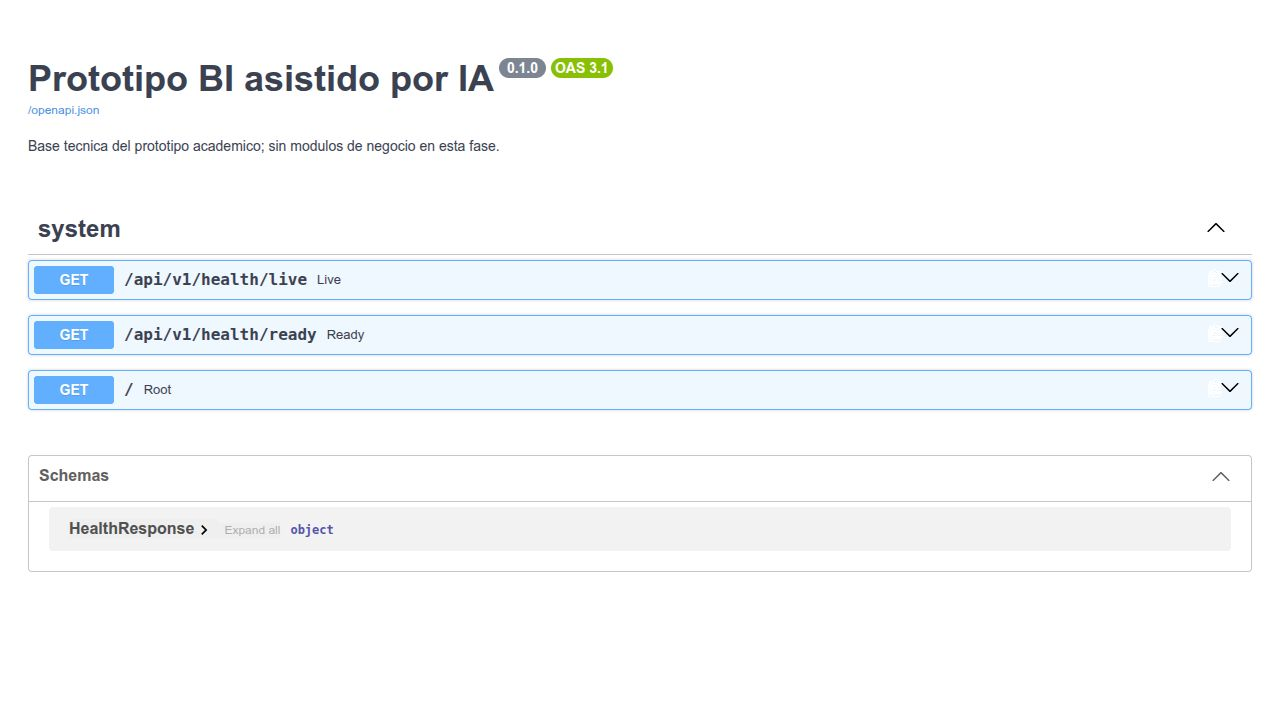
\includegraphics[width=\textwidth]{../assets/sprint-01/openapi.jpg}
  \caption{Endpoints técnicos disponibles en el Sprint 1.}
\end{figure}

\subsection{Validación de AdventureWorks}

La restauración correcta debe producir 71 tablas de usuario. La sonda del contenedor se autentica como \file{bi\_reader}; por tanto, un estado saludable confirma que la cuenta puede conectar y leer.

Para una auditoría explícita, ingresar al contenedor usando variables ya inyectadas y ejecutar consultas controladas. No copiar las contraseñas al historial:

\begin{lstlisting}[style=terminal,language=bash]
docker compose exec sqlserver bash
/opt/mssql-tools18/bin/sqlcmd -S localhost \
  -U "$SQLSERVER_USER" -P "$SQLSERVER_PASSWORD" -C \
  -d "$SQLSERVER_DATABASE" -Q \
  "SELECT COUNT(*) AS tablas FROM sys.tables;"
exit
\end{lstlisting}

No se debe ejecutar una prueba destructiva sobre datos que deban conservarse. La automatización de inicialización ya verifica las denegaciones de escritura de forma controlada.

\section{Operación completa de los contenedores}

Todos los comandos de esta sección se ejecutan desde la raíz del repositorio. En este computador:

\begin{lstlisting}[style=terminal,language=bash]
cd "/home/ceo/Proyectos/BI"
\end{lstlisting}

En otro equipo se sustituye esa ruta por la carpeta donde se clonó el repositorio.

\subsection{Diferencia entre pausar, reanudar y retirar}

\begin{tabularx}{\textwidth}{@{}p{0.19\textwidth}p{0.29\textwidth}X@{}}
  \toprule
  Acción & Comando Compose & Efecto \\
  \midrule
  Pausar & \file{docker compose stop} & Detiene los procesos, pero conserva contenedores, red y volúmenes. \\
  Reanudar & \file{docker compose start} & Inicia contenedores existentes sin reconstruir imágenes. Sólo se usa después de \file{stop}. \\
  Retirar & \file{docker compose down} & Retira contenedores y red; conserva los volúmenes nombrados y, por tanto, los datos. \\
  Reiniciar limpio & \file{docker compose down --volumes} & Retira también los volúmenes. Borra las bases del proyecto y obliga a restaurarlas. \\
  \bottomrule
\end{tabularx}

\warningbox{No añadir \file{--volumes} para una detención normal. PostgreSQL y AdventureWorks sólo se conservan cuando los volúmenes permanecen.}

\subsection{Ciclo del ambiente de desarrollo}

El ambiente de desarrollo contiene \file{frontend}, \file{backend}, \file{postgres} y \file{sqlserver}. El perfil opcional \file{local-llm} puede añadir \file{ollama}.

\textbf{Construir y levantar:}

\begin{lstlisting}[style=terminal,language=bash]
make up
make ps
\end{lstlisting}

\textbf{Pausar y reanudar los mismos contenedores:}

\begin{lstlisting}[style=terminal,language=bash]
docker compose stop
docker compose start
\end{lstlisting}

\textbf{Retirar los contenedores y la red, conservando las bases:}

\begin{lstlisting}[style=terminal,language=bash]
make down
\end{lstlisting}

Después de \file{make down}, \file{docker compose start} ya no aplica porque los contenedores fueron retirados. Para crearlos nuevamente se usa \file{make up}; los volúmenes existentes se reutilizan.

\subsection{Ciclo del LLM local opcional}

\begin{lstlisting}[style=terminal,language=bash]
make ollama-up
make ollama-pull
make ollama-status
make ollama-down
\end{lstlisting}

La secuencia inicia el servicio, descarga el modelo una única vez, lista lo disponible y finalmente detiene sólo Ollama. El último comando conserva el volumen \file{ollama\_models}. El perfil no publica el puerto 11434, no se inicia al levantar desarrollo normal y no forma parte de \file{compose.release.yaml}; por ello no cambia la superficie de red de una entrega ni agrega una descarga pesada a CI.

\subsection{Ciclo de la vista local de entrega}

La vista ligera contiene sólo \file{frontend-delivery}; comparte la API, la red y las bases del desarrollo.

\textbf{Construir y levantar Nginx en 8080:}

\begin{lstlisting}[style=terminal,language=bash]
make delivery-preview-up
docker compose --profile delivery ps
\end{lstlisting}

\textbf{Pausar y reanudar únicamente \file{frontend-delivery}:}

\begin{lstlisting}[style=terminal,language=bash]
docker compose --profile delivery stop frontend-delivery
docker compose --profile delivery start frontend-delivery
\end{lstlisting}

\textbf{Detener y retirar únicamente ese contenedor:}

\begin{lstlisting}[style=terminal,language=bash]
docker compose --profile delivery rm --stop --force frontend-delivery
\end{lstlisting}

Estas acciones no detienen Vite, FastAPI, PostgreSQL ni SQL Server. Para volver a crear la vista después de retirarla se ejecuta de nuevo \file{make delivery-preview-up}.

\subsection{Ciclo de la entrega completa desde GHCR}

Este ambiente usa \file{compose.release.yaml}, el proyecto aislado \file{bi-ia-prototype-release} y el archivo \file{.env.release}.

\textbf{Descargar y levantar las cinco imágenes:}

\begin{lstlisting}[style=terminal,language=bash]
make release-up
docker compose --env-file .env.release \
  -f compose.release.yaml ps
\end{lstlisting}

\textbf{Pausar y reanudar sin retirar contenedores:}

\begin{lstlisting}[style=terminal,language=bash]
docker compose --env-file .env.release \
  -f compose.release.yaml stop
docker compose --env-file .env.release \
  -f compose.release.yaml start
\end{lstlisting}

\textbf{Retirar sólo la entrega completa y conservar sus bases:}

\begin{lstlisting}[style=terminal,language=bash]
make release-down
\end{lstlisting}

Los comandos de entrega no afectan los contenedores ni los volúmenes de desarrollo. La vista Nginx ligera y la entrega completa usan 8080 por defecto; no deben levantarse simultáneamente sin cambiar uno de los puertos.

\subsection{Detener todos los ambientes conservando datos}

Si están activos desarrollo, la vista Nginx y la entrega completa:

\begin{lstlisting}[style=terminal,language=bash]
docker compose --profile delivery down
make release-down
\end{lstlisting}

El primer comando retira desarrollo y \file{frontend-delivery}; el segundo retira el proyecto de entrega completo. Ninguno usa \file{--volumes}. Si nunca se configuró \file{.env.release}, se omite \file{make release-down}.

\subsection{Referencia de comandos abreviados}

\begin{tabularx}{\textwidth}{@{}l X@{}}
  \toprule
  Comando & Función \\
  \midrule
  \file{make bootstrap} & Prepara secretos locales, construye y espera la salud del primer arranque. \\
  \file{make up} & Construye cambios y levanta desarrollo en segundo plano. \\
  \file{make delivery-preview-up} & Añade Nginx en 8080 y conserva Vite en 5173. \\
  \file{make ollama-up} & Inicia Ollama local opcional sin descargar un modelo. \\
  \file{make ollama-pull} & Descarga \file{OLLAMA\_MODEL} una vez por equipo. \\
  \file{make ollama-status} & Lista los modelos presentes en el volumen local. \\
  \file{make ollama-down} & Detiene Ollama y conserva el modelo. \\
  \file{make release-up} & Descarga y levanta las cinco imágenes en un proyecto aislado. \\
  \file{make release-down} & Retira sólo la entrega completa y conserva sus volúmenes. \\
  \file{make down} & Retira desarrollo y su red, conservando los volúmenes. \\
  \file{make ps} & Muestra servicios de desarrollo y estado de salud. \\
  \file{make logs} & Sigue los registros recientes. \\
  \file{make test} & Ejecuta pruebas en las etapas Docker de backend y frontend. \\
  \file{make lint} & Ejecuta Ruff, Mypy y ESLint en contenedores. \\
  \file{make compose-check} & Valida Compose de desarrollo, entrega y perfil Ollama opcional. \\
  \file{make docs} & Regenera bitácora, informes de Sprint 1 y Sprint 2, y manual. \\
  \file{make verify} & Ejecuta la verificación completa antes de entregar. \\
  \bottomrule
\end{tabularx}

La recarga automática de Vite y FastAPI permite editar código sin instalar sus dependencias en el host.

\section{Persistencia y reinicio de datos}

\subsection{Detener sin borrar}

\begin{lstlisting}[style=terminal,language=bash]
docker compose --profile delivery down
make release-down
\end{lstlisting}

El primer comando cubre desarrollo y la vista Nginx cuando está activa. El segundo cubre la entrega completa aislada. Los volúmenes permanecen y el siguiente arranque reutiliza PostgreSQL y AdventureWorks.

\subsection{Reconstruir desde cero}

\warningbox{El siguiente procedimiento elimina de forma irreversible sólo los volúmenes del proyecto Compose actual. Confirmar que no contienen resultados que deban conservarse.}

\begin{lstlisting}[style=terminal,language=bash]
docker compose down --volumes
make bootstrap
\end{lstlisting}

La restauración de AdventureWorks volverá a descargar el respaldo cuando el volumen esté vacío.

\subsection{Qué se versiona}

\begin{itemize}
  \item Se versionan Dockerfiles, Compose, scripts, migraciones, documentación y datos sintéticos aprobados.
  \item No se versionan volúmenes, contraseñas, tokens, archivos \file{.bak}, \file{.dump} ni datos productivos.
  \item AdventureWorks se reconstruye desde el respaldo oficial y PostgreSQL desde scripts/migraciones.
\end{itemize}

\section{Actualización y reversión}

\subsection{Entorno construido desde código}

\begin{lstlisting}[style=terminal,language=bash]
git pull --ff-only
docker compose up --build -d
make doctor
\end{lstlisting}

\subsection{Entorno basado en GHCR}

\begin{lstlisting}[style=terminal,language=bash]
docker compose --env-file .env.release -f compose.release.yaml pull
docker compose --env-file .env.release -f compose.release.yaml up -d
\end{lstlisting}

Para volver a una versión conocida, fijar \file{IMAGE\_TAG} a una etiqueta anterior y repetir \file{pull}/\file{up}. No usar \file{latest} para entregas evaluables.

Cuando existan migraciones de datos, la reversión deberá seguir el procedimiento de la versión específica. Nunca sustituir una migración por la copia manual de un volumen.

\section{Flujo Git y CI/CD}

\subsection{Desarrollo por rama}

La rama predeterminada \file{develop} integra el trabajo diario y \file{main} conserva únicamente entregas estables. Las ramas de trabajo parten de \file{develop} con los prefijos \file{feature/}, \file{fix/}, \file{docs/} o \file{chore/}.

\begin{lstlisting}[style=terminal,language=bash]
git switch develop
git pull --ff-only origin develop
git switch -c feature/nombre-cambio
# editar y comprobar
make verify
git add .
git commit -m "feat: descripcion breve"
git push -u origin feature/nombre-cambio
gh pr create --base develop --fill
\end{lstlisting}

El pull request hacia \file{develop} exige CI aprobada, una revisión y conversaciones resueltas. Cuando la iteración sea estable, se abre un segundo pull request de \file{develop} hacia \file{main}; esa promoción vuelve a ejecutar CI y, al fusionarse, activa CD. El procedimiento completo está en \file{docs/git-workflow.md}.

Las ramas \file{develop} y \file{main} tienen protección activa: impiden force-push y eliminación, exigen pull request, una aprobación, conversaciones resueltas y ocho controles de CI con la rama actualizada. La excepción administrativa se reserva para recuperación y debe justificarse en la bitácora.

\subsection{Integración continua}

En cada push y pull request hacia \file{develop} o \file{main}, CI:

\begin{enumerate}
  \item valida que los PR de trabajo lleguen a \file{develop} y que sólo \file{develop} promueva a \file{main};
  \item valida el archivo Compose;
  \item construye la etapa de prueba del backend;
  \item construye la etapa de prueba del frontend;
  \item construye las imágenes de infraestructura;
  \item compila los documentos LaTeX y verifica que los PDF versionados estén actualizados.
\end{enumerate}

Los trabajos de CI son efímeros: construyen y prueban contenedores en GitHub y los eliminan al terminar. No mantienen un servidor de desarrollo ni modifican los ambientes locales de los colaboradores.

\subsection{Entrega continua}

Después de un cambio en \file{main} o una etiqueta \file{v*}, CD valida y publica:

\begin{itemize}
  \item \file{prototipo-bi-ia-backend};
  \item \file{prototipo-bi-ia-frontend};
  \item \file{prototipo-bi-ia-postgres};
  \item \file{prototipo-bi-ia-sqlserver};
  \item \file{prototipo-bi-ia-docs}.
\end{itemize}

Las ejecuciones de línea base CI 32749237009 y CD 32749237059 finalizaron exitosamente para el commit \file{ddf2551}.

CD tampoco reemplaza automáticamente un servidor: publica imágenes con etiquetas \file{main}, \file{sha-*} y \file{v*}. Cada computador o proveedor de despliegue selecciona una etiqueta mediante \file{.env.release}. Así pueden coexistir desarrollo y producción sin compartir red, puertos ni volúmenes.

\subsection{Cierre propuesto en Azure}

Se recomienda Azure for Students para la demostración académica. La suscripción aporta crédito temporal, no alojamiento gratuito permanente. La arquitectura objetivo usa una VM Ubuntu x64 con 2 vCPU y 8 GiB, Docker Compose, alertas de presupuesto y apagado o desasignación fuera de las pruebas. SQL Server requiere x64 y consume una parte relevante de la memoria; una instancia gratuita mínima no es suficiente para el conjunto completo.

El despliegue seguirá esta secuencia:

\begin{enumerate}
  \item CI aprueba el pull request y la promoción \file{develop -> main};
  \item CD publica las cinco imágenes y una etiqueta inmutable;
  \item el ambiente GitHub \file{production} exige la aprobación definida por el equipo;
  \item GitHub Actions se autentica en Azure mediante OIDC y permisos limitados;
  \item la VM descarga la etiqueta, ejecuta Compose y comprueba salud;
  \item se registran SHA, digest, URL, resultado y cualquier reversión.
\end{enumerate}

La suscripción, la VM y el workflow de despliegue permanecen pendientes hasta que las autoras activen Azure for Students y confirmen región, presupuesto y nombres. No se almacenará una contraseña permanente de Azure en GitHub.

Dependabot trabaja contra la rama predeterminada \file{develop}. Las actualizaciones npm menores y parches se agrupan; los saltos mayores se revisan de forma intencional y separada para evitar mezclar migraciones incompatibles.

\subsection{Cómo verificar CI y CD en GitHub}

En GitHub se abre la pestaña \textbf{Actions}. Cada fila representa una ejecución; el círculo verde significa que todos sus trabajos terminaron correctamente y el rojo identifica una ejecución que necesita revisión. Al abrir una ejecución se puede leer cada trabajo, descargar los artefactos de documentación y conservar el enlace como evidencia para la tesis.

\begin{figure}[H]
  \centering
  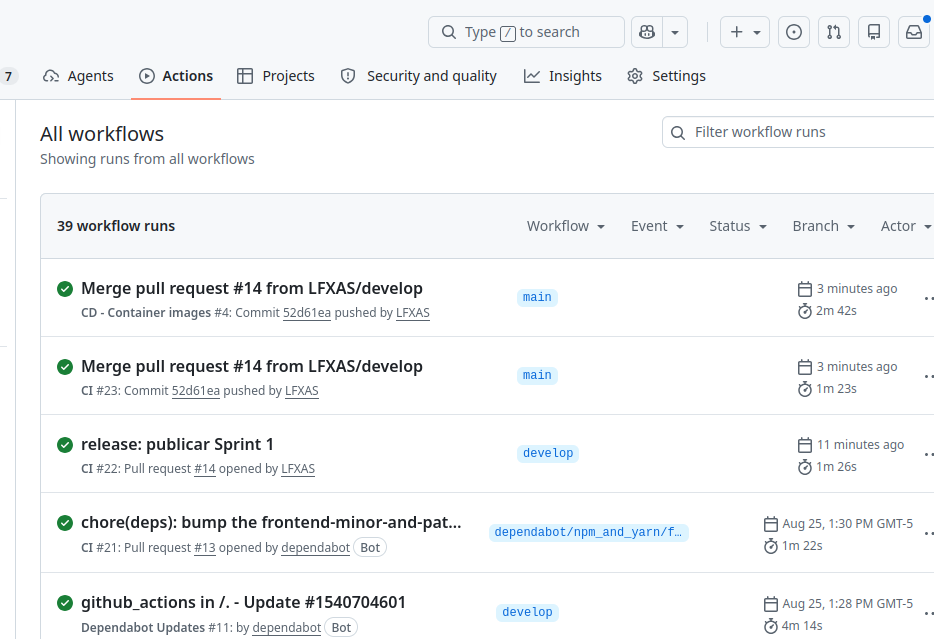
\includegraphics[width=0.96\textwidth]{../assets/sprint-01/github-actions.png}
  \caption{Historial real de GitHub Actions: CI y CD concluyen con estado satisfactorio después de promover \file{develop} hacia \file{main}.}
\end{figure}

\begin{tabularx}{\textwidth}{@{}p{0.22\textwidth}X X@{}}
  \toprule
  Flujo & Cuándo se ejecuta & Resultado esperado \\
  \midrule
  CI & Push o pull request hacia \file{develop} o \file{main}. & Valida flujo de ramas, Compose, backend, frontend, infraestructura y los cuatro PDF. No publica ni deja contenedores activos ni descarga modelos LLM. \\
  CD & Cambio ya fusionado en \file{main} o etiqueta \file{v*}. & Revalida backend/frontend y publica cinco imágenes de producción en GHCR con etiqueta de rama, SHA y, cuando aplique, versión. No despliega aún una VM Azure. \\
  Dependabot & Según su programación. & Abre un PR temporal de actualización; se revisa y prueba igual que un cambio humano. \\
  \bottomrule
\end{tabularx}

Para diagnosticar una falla se abre primero el trabajo con marca roja, se identifica el paso que falló y se reproduce localmente con \file{make verify} desde la raíz del repositorio. No se fusiona un PR fallido ni se intenta corregir modificando directamente \file{main}. Un cambio documental también pasa por CI porque los PDF versionados deben coincidir con sus fuentes \LaTeX.

\begin{figure}[H]
  \centering
  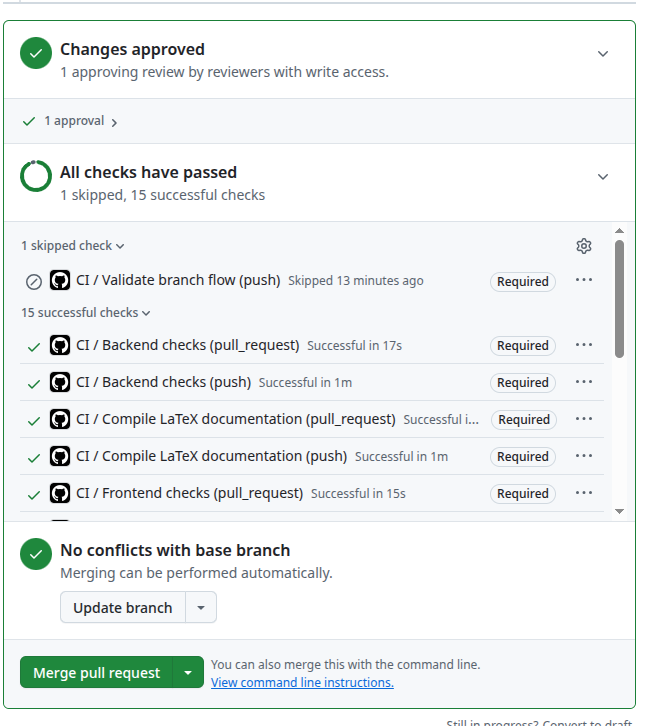
\includegraphics[height=0.57\textheight]{../assets/sprint-01/pr-checks.png}
  \caption{Control de promoción: aprobación humana, verificaciones obligatorias y ausencia de conflictos antes de habilitar la fusión.}
\end{figure}

\subsection{Qué significa DevOps en este prototipo}

DevOps no es un contenedor adicional ni una persona distinta. En este proyecto es la práctica de mantener código, infraestructura, pruebas, documentación y entrega dentro del mismo ciclo trazable. Docker evita diferencias entre computadoras; Git conserva el historial; pull requests y protecciones controlan la revisión; CI comprueba cada integración; CD crea imágenes reutilizables; GHCR permite descargarlas; la bitácora y los PDF conservan la evidencia.

El responsable integrador trabaja en una rama de función, corre las verificaciones y abre el PR. Las colaboradoras pueden reproducir el ambiente, revisar, documentar y aprobar. Sólo la promoción aprobada de \file{develop} a \file{main} representa una entrega estable. GitHub Actions inicia CD automáticamente después de esa fusión: no hay que presionar un botón de despliegue local y tampoco se modifica una instalación de otra persona.

\section{Desarrollo guiado por especificaciones (SDD)}

\textbf{SDD} significa \emph{Specification-Driven Development}: antes de programar una capacidad se escribe una especificación breve, verificable y versionada. La intención es evitar que una idea, una propuesta de IA o un cambio de datos se transforme en código sin que el equipo haya acordado su alcance, sus límites y la evidencia que demostrará que funciona.

El Sprint 1 no se rehace con SDD porque ya se cerró como una base técnica. Desde el Sprint 2 la especificación es obligatoria para toda capacidad funcional nueva. Los archivos se conservan en \file{docs/specs/}; la guía es \file{docs/sdd-workflow.md} y \file{docs/specs/TEMPLATE.md} contiene la plantilla.

\subsection{Procedimiento SDD para cada función}

\begin{enumerate}
  \item Copiar la plantilla y crear un archivo con el identificador del sprint. Por ejemplo: \path{SPR-02-rbac-y-parametros.md}.
  \item Escribir el problema, objetivo, alcance incluido, exclusiones, actores, datos, API/interfaz, seguridad, criterios de aceptación, pruebas, riesgos y dependencias.
  \item Revisar y aprobar la especificación antes de implementar. Si la decisión afecta permanentemente la arquitectura, crear además un ADR en \file{docs/decisions/}.
  \item Crear la rama desde \file{develop}, implementar dentro del alcance y enlazar la especificación en el PR.
  \item Añadir pruebas; actualizar README, arquitectura, réplica, manual y bitácora cuando resulte afectado; ejecutar \file{make verify}.
  \item Con CI verde y revisión aprobada, fusionar hacia \file{develop}. Registrar el PR, SHA, evidencia y desviaciones en la bitácora.
  \item Promover \file{develop} hacia \file{main} únicamente cuando el incremento integrado sea estable. CD publicará las imágenes sin sustituir los volúmenes ni los equipos de desarrollo.
\end{enumerate}

\notebox{La especificación no sustituye las pruebas. Define qué se debe probar. En especial, cualquier propuesta de IA, SQL o ETL debe declarar aprobación humana, validaciones determinísticas, datos permitidos y auditoría antes de ejecutarse.}

\clearpage
\section{Construcción operativa del Sprint 1 desde cero}

Esta sección explica cómo se concibió la línea base del Sprint 1 y qué debe realizar una persona para reconstruirla manualmente. No sustituye los archivos versionados: los interpreta, relaciona y ordena. Los comandos se ejecutan desde la raíz del repositorio, salvo que se indique otra ruta.

\subsection{Secuencia de construcción}

\begin{enumerate}
  \item Revisar el alcance y separar infraestructura de funcionalidades. En el Sprint 1 sólo se autorizaron salud técnica, estructura modular, contenedores, repositorio, automatización y documentación.
  \item Crear las carpetas \file{backend}, \file{frontend}, \file{infra}, \file{scripts}, \file{docs} y \file{.github/workflows}. Esta separación permite construir y probar cada componente de manera independiente.
  \item Preparar Dockerfiles multietapa. Las etapas \file{development}, \file{test} y \file{production} evitan usar una imagen de desarrollo como entrega estable.
  \item Definir \file{compose.yaml} como orquestador local y \file{compose.release.yaml} como consumidor de imágenes publicadas. Cada uno usa nombre, puertos, red y volúmenes independientes.
  \item Crear \file{.env.example} y \file{.env.release.example}; mantener los archivos reales fuera de Git.
  \item Implementar sondas de salud y dependencias condicionadas. El frontend no debe declararse listo antes del backend; FastAPI no debe iniciar antes de las bases saludables.
  \item Incorporar scripts idempotentes para crear esquemas PostgreSQL y restaurar la fuente SQL Server. Repetir un arranque no debe duplicar objetos ni corromper datos.
  \item Centralizar operaciones repetidas en el \file{Makefile}: levantar, verificar, compilar documentación y ejecutar pruebas.
  \item Inicializar Git, crear \file{develop} y \file{main}, configurar colaboradores y aplicar protección de ramas.
  \item Crear CI para validar cada cambio y CD para publicar sólo aquello que ya llegó a \file{main} o a una etiqueta \file{v*}.
  \item Ejecutar una prueba limpia, registrar incidentes y conservar PDF, commit, Action y digest como evidencia.
\end{enumerate}

\subsection{Primera instalación manual reproducible}

\begin{lstlisting}[style=terminal,language=bash]
git clone https://github.com/LFXAS/prototipo-bi-ia.git
cd prototipo-bi-ia
git switch develop
cp .env.example .env
# Editar .env y sustituir cada ChangeMe_*
docker compose config --quiet
docker compose build
docker compose up -d
docker compose ps
curl --fail http://localhost:8000/api/v1/health/live
curl --fail http://localhost:8000/api/v1/health/ready
\end{lstlisting}

\file{docker compose config --quiet} detecta variables o estructuras YAML inválidas antes de consumir tiempo construyendo imágenes. \file{build} procesa los Dockerfiles y crea capas locales. \file{up -d} crea la red, los volúmenes y los contenedores en segundo plano. \file{ps} permite comprobar estado y salud. Las dos peticiones HTTP distinguen entre proceso vivo y dependencias realmente disponibles.

\section{Referencia comentada de configuración}

\subsection{Archivos de entorno}

\file{.env.example} es una plantilla versionable para desarrollo. El archivo real \file{.env} es local. Sus grupos tienen estas funciones:

\begin{itemize}
  \item \file{COMPOSE\_PROJECT\_NAME}: crea un espacio de nombres y evita mezclar redes, volúmenes y contenedores con otros proyectos.
  \item \file{FRONTEND\_PORT}, \file{DELIVERY\_FRONTEND\_PORT} y \file{BACKEND\_PORT}: publican servicios web en el computador anfitrión.
  \item \file{LOCAL\_POSTGRES\_PORT} y \file{LOCAL\_SQLSERVER\_PORT}: permiten inspección local; dentro de Docker se siguen usando 5432 y 1433.
  \item \file{POSTGRES\_*}: identifican la base interna y su cuenta de aplicación.
  \item \file{SQLSERVER\_*}: identifican la fuente externa, la cuenta lectora, el controlador y las opciones cifradas.
  \item \file{VITE\_API\_BASE\_URL}: vacía hace que Vite o Nginx envíe \file{/api} al backend sin fijar una dirección del host en el código compilado.
\end{itemize}

\file{.env.release.example} usa puertos distintos y añade \file{IMAGE\_PREFIX} y \file{IMAGE\_TAG}. El prefijo apunta a GHCR y la etiqueta decide qué entrega se ejecuta. \file{main} es móvil; una etiqueta como \file{v0.1.0} es la opción adecuada para una evidencia inmutable.

\begin{lstlisting}[style=terminal]
IMAGE_PREFIX=ghcr.io/lfxas/prototipo-bi-ia
IMAGE_TAG=main
\end{lstlisting}

Los valores \file{ChangeMe\_*} son marcadores, no contraseñas válidas para una entrega. La plantilla puede versionarse porque no concede acceso. Los archivos reales deben aparecer ignorados por Git y comprobarse antes de cada commit con \file{git status} y, cuando sea necesario, \file{git diff --cached}.

\subsection{Compose de desarrollo: \file{compose.yaml}}

La clave \file{name} fija el nombre lógico del proyecto. \file{services} describe los cinco servicios posibles; \file{volumes} declara persistencia administrada por Docker.

\begin{longtable}{@{}p{0.20\textwidth}p{0.30\textwidth}p{0.42\textwidth}@{}}
  \toprule
  \textbf{Bloque} & \textbf{Directiva relevante} & \textbf{Razón técnica} \\
  \midrule
  \endfirsthead
  \toprule
  \textbf{Bloque} & \textbf{Directiva relevante} & \textbf{Razón técnica} \\
  \midrule
  \endhead
  PostgreSQL & \file{build}, \file{environment}, \file{volumes} & Construye la imagen propia, inicializa los esquemas y conserva los datos fuera del ciclo de vida del contenedor. \\
  PostgreSQL & \file{healthcheck} con \file{pg\_isready} & Confirma que el motor acepta conexiones antes de habilitar dependientes. \\
  SQL Server & \file{platform: linux/amd64} & Declara la arquitectura compatible con la imagen de SQL Server. \\
  SQL Server & \file{ADVENTUREWORKS\_BACKUP\_URL} & Permite restaurar el respaldo oficial al iniciar un volumen vacío, sin versionar el archivo \file{.bak}. \\
  SQL Server & archivo de marca y \file{sqlcmd} & La salud exige restauración terminada y conexión real del usuario lector. \\
  Backend & etapa \file{development} y montaje \file{./backend:/app} & Activa recarga automática y refleja cambios del editor sin copiar manualmente archivos. \\
  Backend & \file{depends\_on: condition: service\_healthy} & Evita iniciar FastAPI cuando las bases todavía no están listas. \\
  Frontend & montaje del código y volumen \file{node\_modules} & Conserva dependencias Linux dentro de Docker y permite recarga de Vite. \\
  Entrega local & \file{profiles: [delivery]} & Nginx sólo se crea cuando se solicita; no consume recursos durante desarrollo ordinario. \\
  Todos & \file{restart: unless-stopped} & Reinicia después de una falla o reinicio del daemon, excepto cuando la persona los detuvo expresamente. \\
  \bottomrule
\end{longtable}

La sintaxis \file{\${VARIABLE:-valor}} significa usar la variable del entorno si existe y, de lo contrario, emplear el valor indicado. La forma \file{\$\$VARIABLE} escapa el signo para que Compose lo entregue al contenedor y sea el shell interno quien lo interprete.

\subsection{Compose de producción local: \file{compose.prod.yaml}}

Este archivo es una sobreescritura para construir las etapas \file{production} de backend y frontend. Desactiva los montajes de código y la depuración, utiliza Nginx y aplica una política de reinicio más estricta. Se conserva como configuración de construcción; la réplica publicada usa \file{compose.release.yaml}.

\subsection{Compose de entrega: \file{compose.release.yaml}}

La diferencia esencial es \file{image} en lugar de \file{build}. El equipo receptor descarga las cinco imágenes ya verificadas desde GHCR. El proyecto predeterminado \file{bi-ia-prototype-release}, los puertos 8080, 18000, 55433 y 51434 y los volúmenes propios permiten ejecutar desarrollo y entrega a la vez. No se trasladan bases mediante volúmenes: PostgreSQL se inicializa o migra y la fuente de demostración se restaura de forma reproducible.

\begin{lstlisting}[style=terminal,language=bash]
cp .env.release.example .env.release
# Cambiar secretos y seleccionar IMAGE_TAG
docker compose --env-file .env.release \
  -f compose.release.yaml pull
docker compose --env-file .env.release \
  -f compose.release.yaml up -d
\end{lstlisting}

\subsection{Dockerfile del backend}

El backend usa una construcción multietapa:

\begin{enumerate}
  \item \file{base}: parte de Python slim, instala certificados, ODBC y el controlador Microsoft; copia metadatos y aplicación.
  \item \file{development}: instala dependencias de desarrollo y ejecuta Uvicorn con \file{--reload}.
  \item \file{test}: copia las pruebas y obliga a pasar Ruff, comprobación de formato, Mypy y Pytest durante la construcción.
  \item \file{production}: instala sólo el paquete, crea un usuario sin privilegios y ejecuta dos trabajadores sin recarga ni depuración.
\end{enumerate}

El patrón hace que una imagen de pruebas no pueda terminar correctamente si falla una comprobación. CI aprovecha esa propiedad construyendo directamente \file{target: test}.

\subsection{Dockerfile del frontend}

\file{dependencies} ejecuta \file{npm ci} a partir del lockfile, lo que reproduce versiones exactas. \file{development} inicia Vite escuchando en todas las interfaces del contenedor. \file{test} ejecuta ESLint, Vitest y la compilación. \file{build} genera archivos estáticos. \file{production} parte de Nginx y copia solamente \file{dist}; por ello no incluye Node.js ni el código fuente de desarrollo durante la entrega.

\subsection{Imágenes de infraestructura}

\begin{itemize}
  \item \path{infra/postgres/Dockerfile}: extiende PostgreSQL y copia scripts SQL a \path{/docker-entrypoint-initdb.d/}. Esos scripts se ejecutan sólo al inicializar un volumen vacío.
  \item \file{infra/sqlserver/Dockerfile}: extiende SQL Server 2022, instala herramientas de descarga y configura un punto de entrada que levanta el motor y ejecuta la restauración idempotente.
  \item \file{infra/docs/Dockerfile}: fija Debian, \file{latexmk} y paquetes TeX. Gracias a esta imagen, el PDF se construye igual en estaciones y GitHub Actions.
\end{itemize}

\section{Automatización local con Make y scripts}

Make no reemplaza Docker Compose; proporciona nombres estables para secuencias largas.

\begin{longtable}{@{}p{0.25\textwidth}p{0.67\textwidth}@{}}
  \toprule
  \textbf{Objetivo} & \textbf{Acción y uso} \\
  \midrule
  \endfirsthead
  \toprule
  \textbf{Objetivo} & \textbf{Acción y uso} \\
  \midrule
  \endhead
  \file{make env} & Crea \file{.env} sólo cuando todavía no existe; no sobrescribe secretos locales. \\
  \file{make bootstrap} & Ejecuta la preparación inicial, el arranque y la espera controlada de todos los servicios. \\
  \file{make up}/\file{make down} & Construye y levanta desarrollo o retira contenedores y red conservando volúmenes. \\
  \file{make delivery-preview-up} & Construye Nginx y añade sólo la vista de entrega al ambiente de desarrollo. \\
  \file{make release-up}/\file{make release-down} & Descarga, inicia o retira el ambiente GHCR usando el archivo de entorno de entrega. \\
  \file{make test} & Construye las etapas de prueba de frontend y backend; un fallo interrumpe el objetivo. \\
  \file{make lint} & Ejecuta Ruff, Mypy y ESLint dentro de contenedores desechables. \\
  \file{make compose-check} & Valida desarrollo, perfil de entrega y entrega GHCR sin iniciar servicios. \\
  \file{make docs} & Construye la imagen LaTeX y regenera bitácora, informe y manual. \\
  \file{make verify} & Agrupa configuración, política de ramas, pruebas y documentos; es la puerta local antes del push. \\
  \bottomrule
\end{longtable}

Los scripts de \file{scripts/} resuelven operaciones que Compose no expresa por sí solo: preparar el archivo de entorno, esperar salud con límite de tiempo, verificar endpoints, validar la dirección de las ramas y probar esa política con casos permitidos y prohibidos.

\section{Git y GitHub: procedimiento completo}

\subsection{Inicialización conceptual del repositorio}

En un proyecto nuevo, la secuencia manual equivalente es:

\begin{lstlisting}[style=terminal,language=bash]
git init -b main
git add .
git commit -m "chore: initialize reproducible environment"
git switch -c develop
git remote add origin URL_DEL_REPOSITORIO
git push -u origin main
git push -u origin develop
\end{lstlisting}

En este repositorio esa inicialización ya se realizó. No debe repetirse dentro de un clon. Una programadora actualiza sus carpetas con \file{fetch}, \file{switch} y \file{pull --ff-only}; no vuelve a clonar cada vez.

\subsection{Trabajo diario y revisión}

\begin{lstlisting}[style=terminal,language=bash]
git fetch --prune origin
git switch develop
git pull --ff-only origin develop
git switch -c feature/descripcion-breve
# editar archivos
make verify
git status
git diff
git add RUTAS_ESPECIFICAS
git diff --cached
git commit -m "feat: descripcion verificable"
git push -u origin feature/descripcion-breve
\end{lstlisting}

En GitHub se abre un PR con base \file{develop}. Otra persona revisa archivos y evidencia, selecciona \emph{Approve} y la integración sólo se habilita cuando los controles obligatorios están verdes. Para liberar, se abre un segundo PR cuya base es \file{main} y cuyo origen es \file{develop}. Esta separación conserva una rama integradora y otra estable.

\subsection{Protecciones que deben configurarse en GitHub}

Para \file{develop} y \file{main} se requiere PR, una aprobación, conversaciones resueltas, controles vigentes, prohibición de force-push y prohibición de borrar. En \file{main}, la validación adicional rechaza cualquier PR cuyo origen no sea \file{develop}. Estas reglas son controles preventivos; CI aporta el control detectivo.

\section{Integración continua: lectura de \file{ci.yml}}

\subsection{Disparadores, concurrencia y permisos}

\begin{lstlisting}[style=terminal]
on:
  push:
    branches: [main, develop]
  pull_request:
    branches: [main, develop]
concurrency:
  group: ci-${{ github.ref }}
  cancel-in-progress: true
permissions:
  contents: read
\end{lstlisting}

CI se ejecuta en pushes y PR relacionados con las ramas permanentes. La agrupación cancela una ejecución anterior de la misma referencia cuando llega un commit nuevo. El permiso \file{contents: read} aplica privilegio mínimo: CI puede leer el código, pero no modificarlo ni publicar paquetes.

\subsection{Trabajos y dependencia entre resultados}

\begin{itemize}
  \item \file{branch-flow}: sólo en PR; prueba el validador y comprueba base/origen reales.
  \item \file{compose}: interpreta las tres configuraciones para detectar errores antes de construir.
  \item \file{backend}: construye \file{target: test}; Ruff, formato, Mypy y Pytest están incorporados en esa etapa.
  \item \file{frontend}: construye \file{target: test}; ejecuta lint, pruebas y compilación.
  \item \file{infrastructure}: una matriz construye PostgreSQL, SQL Server y LaTeX en paralelo sin publicar.
  \item \file{documentation}: compila los tres PDF, exige que coincidan con los archivos versionados y los adjunta como artefacto de la ejecución.
\end{itemize}

\file{actions/checkout} descarga el commit dentro del ejecutor temporal. \file{setup-buildx} habilita el constructor moderno y caché. \file{build-push-action} construye sin publicar porque \file{push: false}. \file{cache-from} y \file{cache-to} reducen tiempo, pero no sustituyen pruebas.

El paso \file{git diff --exit-code} de documentación detecta un error frecuente: modificar LaTeX sin regenerar el PDF. \file{upload-artifact} permite descargar el conjunto documental desde la ejecución de Actions.

\section{Entrega continua: lectura de \file{cd.yml}}

CD se dispara después de un push a \file{main} o de una etiqueta que comience con \file{v}. No se dispara directamente desde una rama \file{feature/*}. La concurrencia no cancela una publicación en marcha, lo que evita dejar una entrega incompleta.

\begin{lstlisting}[style=terminal]
permissions:
  contents: read
  packages: write
\end{lstlisting}

El token efímero \file{GITHUB\_TOKEN} puede leer el repositorio y escribir paquetes, sin almacenar una contraseña personal. El trabajo \file{verify} valida Compose y vuelve a ejecutar las etapas de prueba. \file{publish} declara \file{needs: verify}; por tanto, ninguna imagen se publica si la verificación falla.

La matriz publica cinco componentes. \file{docker/login-action} inicia sesión en GHCR; \file{metadata-action} genera etiquetas de rama, versión y SHA; \file{build-push-action} construye \file{target: production} y ejecuta \file{push: true}. El SHA crea trazabilidad incluso cuando la etiqueta \file{main} avanza.

\subsection{Qué hace y qué no hace el CD actual}

El CD actual produce y publica artefactos ejecutables. Todavía no crea una VM ni actualiza un servidor Azure. Por ello se denomina entrega continua, no despliegue automático completo. Un despliegue futuro debe seleccionar una etiqueta aprobada, autenticarse mediante OIDC, actualizar el Compose remoto, comprobar salud y conservar el digest.

\section{Dependabot y mantenimiento controlado}

\file{dependabot.yml} revisa semanalmente GitHub Actions, Python y npm. El frontend agrupa actualizaciones menores y parches y excluye saltos mayores. Cada propuesta es un PR ordinario: debe pasar CI y ser revisada. Una rama \file{dependabot/*} es temporal y no representa una rama de arquitectura ni un ambiente.

\section{Persistencia, datos y paso a producción}

Una imagen contiene software e inicializadores; un volumen contiene estado. No se publica el volumen de PostgreSQL ni el de SQL Server en GitHub. Para una instalación nueva, PostgreSQL crea su estructura mediante scripts y, desde el Sprint 2, migraciones Alembic. Los datos de prueba no deben migrarse a producción. Los catálogos indispensables se cargarán con semillas idempotentes y la configuración variable se creará mediante CRUD y procesos de puesta en marcha.

El esquema \file{mart} es dinámico: sus estructuras y cargas dependerán del escenario BI aprobado. No debe congelarse un volumen de demostración como si fuera una base productiva. La fuente SQL Server se conecta con una cuenta de sólo lectura y puede residir en la misma LAN, una VPN o una red alcanzable desde el backend; publicar la aplicación en la nube no le concede acceso automático a una base local.

\section{Prueba final y evidencia del Sprint 1}

\begin{lstlisting}[style=terminal,language=bash]
make verify
make bootstrap
docker compose ps
make delivery-preview-up
curl --fail http://localhost:8080
\end{lstlisting}

Se debe conservar: identificador del commit, URL del PR, aprobación, resumen de controles, PDF generado, captura de servicios saludables, pantalla web, OpenAPI, etiquetas y digest de GHCR y resultado de una réplica en otro computador. La captura nunca debe mostrar tokens, contraseñas o el contenido del archivo \file{.env}.

\subsection{Errores de escritura frecuentes}

Las opciones de Git no admiten espacios internos. Los comandos correctos son:

\begin{lstlisting}[style=terminal,language=bash]
git fetch --prune origin
git pull --ff-only origin develop
\end{lstlisting}

Escribir \file{-- prune} hace que Git interprete \file{prune} como un repositorio. Escribir \file{--ff - only} produce una ruta extraña. Los caracteres deformados en mensajes en español indican una configuración de codificación de la terminal; no implican que el repositorio esté dañado.


\section{Seguridad operativa}

\begin{enumerate}
  \item Cambiar todas las credenciales de ejemplo antes del primer arranque.
  \item Mantener \file{.env} fuera de Git y fuera de los documentos.
  \item Usar \file{bi\_reader} para AdventureWorks; no conectar la aplicación como \file{sa}.
  \item Conservar \file{SQLSERVER\_APPLICATION\_INTENT=ReadOnly}, pero apoyarse en permisos reales del motor.
  \item Gestionar la visibilidad de cada paquete GHCR de forma independiente y no incluir secretos ni datos reales en ninguna imagen.
  \item Otorgar acceso únicamente a cuentas identificadas y revocar colaboradores que ya no participen.
  \item Revisar los cambios de Dependabot y no fusionarlos sin CI aprobada.
  \item RBAC ya exige que FastAPI autorice cada endpoint; ocultar menús en React no es un control de seguridad.
\end{enumerate}

\section{Diagnóstico de fallos}

\begin{longtable}{@{}p{0.27\textwidth}p{0.32\textwidth}p{0.34\textwidth}@{}}
  \toprule
  \textbf{Síntoma} & \textbf{Causa probable} & \textbf{Acción recomendada} \\
  \midrule
  \endfirsthead
  \toprule
  \textbf{Síntoma} & \textbf{Causa probable} & \textbf{Acción recomendada} \\
  \midrule
  \endhead
  Puerto ocupado & Otro servicio usa 5173, 8080, 8000, 18000, 55432, 55433, 51433 o 51434. & Cambiar el puerto correspondiente en el archivo de ambiente y reiniciar Compose. \\
  5173 funciona y 8080 no responde & Sólo está iniciado el perfil normal de desarrollo. & Ejecutar \file{make delivery-preview-up} o iniciar la entrega completa. \\
  Backend vivo, pero \file{ready} falla & PostgreSQL no está saludable o las credenciales no coinciden. & Revisar \file{docker compose ps} y los registros de PostgreSQL/backend. \\
  SQL Server no queda saludable & Memoria insuficiente, clave SA inválida o descarga bloqueada. & Asignar 8 GB a Docker, corregir la clave y revisar los registros. \\
  Restauración muy lenta & Primera descarga o emulación ARM. & Esperar y seguir \file{docker compose logs -f sqlserver}. \\
  SQL Server queda no saludable tras reiniciar & AdventureWorks todavía está recuperándose. & Esperar la sonda; el inicializador comprueba la base antes de recrear la marca de disponibilidad. \\
  Frontend no muestra API disponible & Backend no saludable o proxy mal configurado. & Probar \file{/health/live}, revisar puertos y registros del frontend. \\
  GHCR devuelve \file{denied} & Falta autenticación, acceso al paquete o permiso \file{read:packages}. & Repetir \file{docker login ghcr.io} con una cuenta autorizada. \\
  PDF no se actualiza & No se regeneró después de editar LaTeX. & Ejecutar \file{make docs} y revisar los archivos modificados. \\
  CI rechaza el cambio & Pruebas, formato, Compose o PDF desactualizado. & Abrir el trabajo fallido, reproducir con \file{make verify} y corregir antes de fusionar. \\
  \bottomrule
\end{longtable}

\subsection{Registros útiles}

\begin{lstlisting}[style=terminal,language=bash]
docker compose logs --tail=200 backend
docker compose logs --tail=200 frontend
docker compose logs --tail=200 postgres
docker compose logs --tail=200 sqlserver
docker compose --profile local-llm logs --tail=200 ollama
\end{lstlisting}

\section{Lista de comprobación para una demostración}

\begin{enumerate}
  \item Confirmar que el commit o etiqueta corresponde a la entrega evaluada.
  \item Ejecutar \file{make verify} y conservar la evidencia de CI.
  \item Ejecutar \file{docker compose ps}; los cuatro servicios deben estar saludables.
  \item Consultar \file{/health/live} y \file{/health/ready}.
  \item Abrir frontend y OpenAPI en el navegador.
  \item Confirmar que AdventureWorks contiene 71 tablas y el acceso externo usa \file{bi\_reader}.
  \item Confirmar que no hay secretos ni archivos \file{.env} en los cambios de Git.
  \item Registrar SHA, etiqueta y digest de imágenes en la bitácora.
  \item Conservar los PDF generados para la evidencia de tesis.
\end{enumerate}

\section{Mantenimiento de la documentación}

Los documentos se compilan dentro de la imagen \file{bi-ia-docs}; no se instala LaTeX en el host.

\begin{lstlisting}[style=terminal,language=bash]
make logbook
make sprint-report
make sprint2-report
make technical-manual
make docs
\end{lstlisting}

Después de cambios técnicos se deben actualizar, según corresponda, README, arquitectura, guía de réplica, manual técnico, informe del sprint y bitácora. Los PDF finales se versionan; los archivos auxiliares de LaTeX se ignoran.

\section{Responsabilidades y escalamiento}

\begin{tabularx}{\textwidth}{@{}p{0.27\textwidth}X@{}}
  \toprule
  Rol & Responsabilidad \\
  \midrule
  Autoras & Aprobar alcance, secretos, accesos, datos de prueba y entregas académicas. \\
  Colaborador técnico & Trabajar por rama, ejecutar pruebas, actualizar documentación y solicitar revisión. \\
  CI/CD & Repetir controles y publicar imágenes después de la integración autorizada. \\
  FastAPI & Aplica autorización RBAC, validaciones determinísticas, auditoría y pruebas LLM seguras. \\
  Responsable de datos & Confirmar que la fuente externa permanezca en lectura y que no se incorporen datos productivos. \\
  \bottomrule
\end{tabularx}

Ante pérdida de datos locales, credenciales expuestas, imágenes inesperadas o permisos de escritura en AdventureWorks, detener la demostración, conservar registros, revocar las credenciales afectadas y documentar la resolución antes de continuar.

\appendix
\section{Referencia rápida de URLs y puertos}

\begin{tabularx}{\textwidth}{@{}l l X@{}}
  \toprule
  Recurso & Dirección & Observación \\
  \midrule
  Frontend desarrollo & \url{http://localhost:5173} & React/Vite \\
  Frontend entrega & \url{http://localhost:8080} & Nginx local o GHCR \\
  API desarrollo & \url{http://localhost:8000} & FastAPI con recarga \\
  API entrega completa & \url{http://localhost:18000} & FastAPI desde GHCR \\
  OpenAPI & \url{http://localhost:8000/docs} & Contrato interactivo \\
  Salud básica & \url{http://localhost:8000/api/v1/health/live} & Proceso de API \\
  Preparación & \url{http://localhost:8000/api/v1/health/ready} & API y PostgreSQL \\
  PostgreSQL & \file{localhost:55432} & Acceso técnico local \\
  SQL Server & \file{localhost:51433} & Acceso técnico local \\
  \bottomrule
\end{tabularx}

\clearpage
\section{Recuperación mínima}
\thispagestyle{fancy}

Si el entorno queda en un estado desconocido y no existen datos que conservar:

\begin{lstlisting}[style=terminal,language=bash]
cd "/ruta/del/repositorio"
docker compose down --volumes
docker compose build --no-cache
make bootstrap
make verify
\end{lstlisting}

\warningbox{La recuperación elimina los volúmenes del proyecto actual. No ejecutarla como diagnóstico rutinario ni en una carpeta cuya identidad Compose no haya sido confirmada.}

\section{Control del manual}

\begin{tabularx}{\textwidth}{@{}>{\bfseries}p{0.26\textwidth}X@{}}
  \toprule
  Campo & Valor \\
  \midrule
  Estado & Manual acumulativo del Sprint 1, Sprint 2 y primer incremento del Sprint 3; base obligatoria para los módulos posteriores con SDD. \\
  Custodia & Repositorio público \file{LFXAS/prototipo-bi-ia}; escritura restringida a colaboradores. \\
  Audiencia & Autoras, tutor, revisores, colaboradores y lectores académicos. \\
  Actualización & Debe acompañar todo cambio de instalación, puertos, secretos, imágenes, pruebas o recuperación. \\
  Fuente editable & \file{docs/manual-tecnico/manual-tecnico.tex}. \\
  Compilación & \file{make technical-manual} o \file{make docs}. \\
  \bottomrule
\end{tabularx}

\subsection*{Historial de cambios}

\begin{tabularx}{\textwidth}{@{}l l X@{}}
  \toprule
  Versión & Fecha & Cambio \\
  \midrule
  1.0.0 & 24-08-2026 & Primera versión: instalación, réplica, operación, CI/CD, seguridad, diagnóstico y recuperación del ambiente del Sprint 1. \\
  1.1.0 & 24-08-2026 & Flujo \file{feature/*} hacia \file{develop}, promoción a \file{main}, protecciones y política de Dependabot. \\
  1.2.0 & 24-08-2026 & Vista Nginx paralela, entrega GHCR aislada y relación entre ramas, CI/CD y ambientes simultáneos. \\
  1.3.0 & 24-08-2026 & Propuesta de cierre DevOps en Azure for Students con VM x64, OIDC, aprobación y control de crédito. \\
  1.4.0 & 24-08-2026 & Ciclo completo para levantar, pausar, reanudar y retirar desarrollo, vista Nginx y entrega GHCR sin borrar volúmenes. \\
  1.5.0 & 01-09-2026 & Explicación ampliada de CI, CD y DevOps; procedimiento SDD, plantillas versionadas y primera especificación del Sprint 2. \\
  1.6.0 & 02-09-2026 & Reconstrucción operativa del Sprint 1 y referencia comentada de variables, Compose, Dockerfiles, Makefile, Git, GitHub, CI/CD, persistencia y verificación. \\
  1.7.0 & 02-09-2026 & Evidencias visuales de GitHub Actions y de los controles obligatorios de aprobación, CI y fusión. \\
  1.8.0 & 11-09-2026 & Consolidación del Sprint 2: operación JWT/RBAC, navegación, CRUD protegido, auditoría, parámetros, proveedores LLM y perfil Docker local de Ollama con persistencia y validación segura. \\
  1.8.1 & 11-09-2026 & Corrección de eliminación de usuarios temporales: auditoría preservada con etiqueta histórica de actor y referencia nula mediante \file{ON DELETE SET NULL}. \\
  1.9.0 & 18-09-2026 & Credenciales LLM administradas desde la web, cifrado autenticado, volumen de raíz criptográfica y migración reproducible como cierre pendiente del Sprint 2. \\
  2.0.0 & 18-09-2026 & Inicio del Sprint 3: conexión SQL Server administrada desde la web, contraseña cifrada, validación de sólo lectura, activación única y cuatro parámetros tipados. \\
  \bottomrule
\end{tabularx}

\subsection*{Registro de revisión}

\begin{tabularx}{\textwidth}{@{}p{0.24\textwidth}X p{0.18\textwidth}@{}}
  \toprule
  Rol & Nombre y conformidad & Fecha \\
  \midrule
  Autora & \rule{0.90\linewidth}{0.4pt} & \rule{0.85\linewidth}{0.4pt} \\[0.6em]
  Autora & \rule{0.90\linewidth}{0.4pt} & \rule{0.85\linewidth}{0.4pt} \\[0.6em]
  Tutor/revisor & \rule{0.90\linewidth}{0.4pt} & \rule{0.85\linewidth}{0.4pt} \\
  \bottomrule
\end{tabularx}

Las firmas formales pertenecen a la tesis entregada y no se versionan si contienen datos personales cuya distribución no fue autorizada.

\end{document}
